\subsection{Erste Datensammlung und manuelle Aufbereitung}
Für eine möglichst gute Datengrundlage wurde an der B19 im Ort Abtsgmünd (Ostalbkreis) Aufnahmen von insgesamt 21 vorbeifahrenden Kfz gemacht, sowohl von dicht aufeinanderfolgenden, als auch einzelnen Fahrzeugen. Die Straße wurde gewählt, da im näheren Umfeld kaum Bebauung ist, die Reflexionen der Fahrzeuggeräusche verursachen könnte. Es ist zudem wichtig, dass die Straße keine Kurven aufweist, da sonst die Wegänderung vorbeifahrender Fahrzeuge nicht korrekt berechnet werden kann. Als Aufnahmegerät wurde ein Smartphone mit integrierter Rekorder-App verwendet. Die zusammenhängende Aufnahme aller Fahrzeuge wurde anschließend von Hand in einzelne Abschnitte unterteilt und als WAV-Audiodateien gespeichert.

Die Auswertung der Audiodaten geschieht auf Grundlage dieser Dateien, das heißt, es wird vorerst \emph{keine} Echtzeitauswertung durchgeführt.

\subsection{Analyse der Audiodaten via Dopplereffekt}
Da im Phy\-sik-Unter\-richt eine Abituraufgabe zur Geschwindigkeitsbestimmung eines Rennwagens mittels Differenz der Frequenz bei Annäherung und Entfernung behandelt wurde, ist das der erste verfolgte Ansatz. Es erscheint zudem einfach, die Geschwindigkeit akkurat zu ermitteln, da selbst ein Mensch eindeutige Frequenzveränderungen hören kann, beispielsweise bei einem vorbeifahrenden Krankenwagen mit Martinshorn. Allerdings muss bei normalen Kfz das Reifengeräusch anstelle des Martinshorns verwendet werden, da dieses mit Abstand die lauteste Geräuschquelle des Straßenverkehrs ist.

Wenn der Abstand des vorbeifahrenden Fahrzeugs zum Beobachter vernachlässigt und von konstanter Bewegungsgeschwindigkeit ausgegangen wird, können folgende Formeln zur Berechnung der Geschwindigkeit verwendet werden:

\[
    f_{1} = f_{0} * \frac{c}{c - v}
    \quad\text{und}\quad
    f_{2} = f_{0} * \frac{c}{c + v}
\]

Dabei ist \(f_{1}\) die vom Beobachter registrierte Frequenz bei Annäherung und \(f_{2}\) die Frequenz bei Entfernung des Fahrzeugs. Die Frequenz \(f_{0}\) stellt die tatsächlich vom Motor generierte Frequenz dar. \cite{PhysikAbituraufgabe}  Die Konstante \(c\) wird mit \(c = 343\frac{m}{s}\) als Schallgeschwindigkeit in Luft definiert. Durch Messung beider Frequenzen kann das Frequenzverhältnis \(k = \frac{f_{1}}{f_{2}}\) berechnet und nach \(v\) umgestellt werden:

\begin{equation*}
    \begin{split}
        k & = \frac{f_{0} * \frac{c}{c - v}}{f_{0} * \frac{c}{c + v}} \\
        k & = \frac{c + v}{c - v} \\
        & \Leftrightarrow \\
        v & = \frac{k - 1}{k + 1} * c
    \end{split}
\end{equation*}

\begin{figure}[h]
    \centering
    \import{rsc/plots/f-t-plot/}{frequenz-zeit-plot.tex}
    \caption{Beispielhafter Frequenzverlauf bei vorbeifahrendem Fahrzeug}
    \label{fig:frequencyplot}
\end{figure}

Des Weiteren ist mit dem Dopplereffekt die Entfernungsbestimmung von Mikrofon und Fahrzeug möglich, indem die Änderungsgeschwindigkeit der Frequenz analysiert wird. Hierbei gilt: je größer die Änderungsrate, desto dichter sind Fahrzeug und Beobachter (siehe \autoref{fig:frequencyplot}).

\subsubsection{Verwendung der Reifengeräusche}

Für einen ersten Überblick wurden die Audio-Abschnitte in einen Spektrumanalysator geladen. Die Ergebnisse der visuellen Analyse sind in \autoref{img:spectrumanalyzer} dargestellt.

\begin{figure}[h]
    \begin{subfigure}{.5\textwidth}
        \centering
        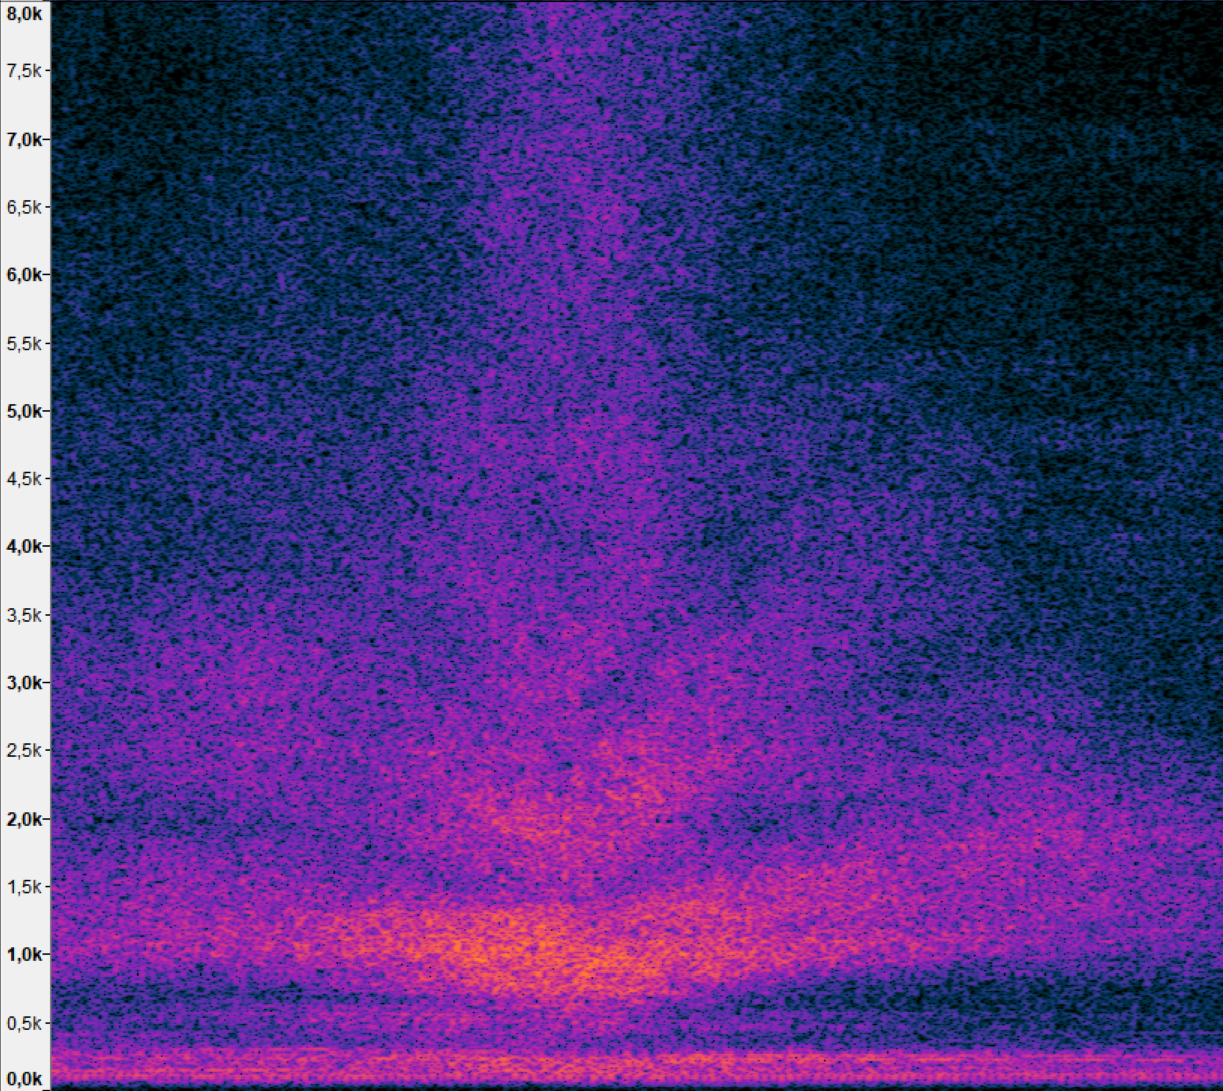
\includegraphics[width=.8\linewidth]{Frequenzen}
        \caption{Spektrogramm}
    \end{subfigure}
    \begin{subfigure}{.5\textwidth}
        \centering
        \includegraphics[width=.8\linewidth]{Tonhöhe(EAC)}
        \caption{Tonhöhe (EAC)}
        \label{img:spectrum_b}
    \end{subfigure}
    \caption{Ergebnisse Spektrumanalysator Reifengeräusche}
    \label{img:spectrumanalyzer}
\end{figure}

Zu \autoref{img:spectrum_b} wurde nachträglich die pinkfarbene Linie hinzugefügt, um den Verlauf der Tonhöhe besser kenntlich zu machen. Diese Linie zeigt den Verlauf der Tonhöhe über Zeit und kann als Frequenzgraph interpretiert werden. An der tiefsten Stelle des Graphen hat das Kfz den geringsten Abstand zum Mikrofon.

Beim Vergleich mit einem theoretisch berechneten Frequenzgraph (\autoref{fig:frequencyplot}) fällt auf, dass die Frequenz der Reifengeräusche nach dem Vorbeifahren (in der Beispielabbildung bei \(t > 10 s\)) niedriger als vor dem Vorbeifahren sein sollte, dies in der Messung aber nicht so ist.

Ich vermute, dass Reflexionen der akustischen Wellen am Boden, die mit den direkt zum Mikrofon laufenden Wellen interferieren und somit hohe Frequenzen auslöschen, die Erklärung für dieses Phänomen sind. Ich konnte bei meiner Recherche keine wissenschaftliche Erarbeitung dieses Phänomens finden. Da mein Ziel die Erstellung der Software ist, habe ich auf eine detaillierte Nachforschung zum jetzigen Zeitpunkt verzichtet.

\subsubsection{Verwendung der Motorgeräusche}

\begin{figure}[h]
    \centering
    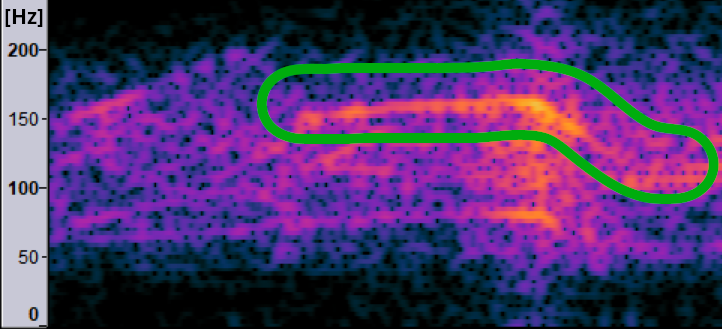
\includegraphics[width=.6\linewidth]{SpektrogrammMotor}
    \caption{Spektrogramm Motorgeräusche}
    \label{fig:spectrum_motor}
\end{figure}

Nachdem sich die Reifengeräusche aufgrund des unerwarteten Tonhöhenverlaufs als unbrauchbar erwiesen haben, ist nun der nächste Ansatz, die Motorgeräusche aufgrund der eindeutigeren Tonhöhe -- anstatt des Rauschens der Reifen -- zu analysieren. Hierfür wird ein Tiefpass mit einer Grenze von \(150 Hz\) auf die Audiospur gelegt, um Reifengeräusche möglichst gut herauszufiltern. Bei der manuellen Analyse stellte sich jedoch heraus, dass selbst die besten Aufnahmen unbrauchbar sind: Der in \autoref{fig:spectrum_motor} grün umrandete Frequenzverlauf stellt die aufgenommenen Motorgeräusche dar, bei denen die Dopplerverschiebung sichtbar ist. Zwar beinhaltet die Aufnahme vor dem Vorbeifahren des Kfz eindeutige Motorgeräusche, allerdings gibt es keine Messpunkte bei Entfernung des Fahrzeugs (hinter dem „Knick“ im Spektrogramm verschwindet die helle, gelbe Linie). Die Motorgeräusche, die direkt mit der Motordrehzahl zusammenhängen, konnten vom verwendeten Handymikrofon gar nicht aufgezeichnet werden, da die Frequenzen unter \(50 Hz\) liegen, das Mikrofon diese Frequenzen jedoch nicht mehr aufnehmen kann. Vermutlich unterläge es jedoch den gleichen Einschränkungen wie die aufgezeichneten Oberwellen. Somit kann auch diese Variante der Geschwindigkeitsbestimmung nicht verwendet werden.

\subsection{Analyse der Audiodaten via Lautstärkeänderung}
\label{section:AnalyseAudiodatenPegel}
Für eine Berechnung der Geschwindigkeit von Fahrzeugen anhand ihrer Lautstärke muss das Verhältnis zwischen Lautstärke und Abstand bekannt sein. Dieses wird im Folgenden mathematisch hergeleitet. Anschließend wird die Anwendbarkeit der Beziehung experimentell erforscht und die Ergebnisse mit der Theorie verglichen.

Die ausschlaggebende Größe für die „Lautstärke“ ist der Schalldruck \(p\), der umgekehrt proportional zur Entfernung \(r\) ist:
\begin{equation}
    p \sim \frac{1}{r}
    \label{equation:reciprocal_distance_law}
\end{equation}

Diese Beziehung wird als reziprokes Abstandsgesetzes bezeichnet. \cite{SengpielSchallpegelEntfernung}
Da der Schalldruck mit einem herkömmlichen Mikrofon jedoch nicht gemessen werden kann, muss eine Umrechnung der aufgenommenen Amplitude auf den Schalldruckpegel (umgangssprachlich oft als „Schallpegel“ bezeichnet) vorgenommen werden. \cite{SchalldruckMessen}
Der Pegel ist immer eine relative Größe, weshalb als Referenzwert die maximal von einer Audiodatei speicherbare Amplitude gewählt wurde.

Aufgrund der logarithmischen Charakteristik eines Pegels \(L_{p}\) kann mittels der Formel für die Pegelberechnung aus der Amplitude \(a mit a \sim p\)
\[
    L_{p} = 20 * \log{\left(a\right)}
\]
hergeleitet werden.

Dieses Verhältnis von Abstand und Pegel kann in die Gleichung
\[
    L_{2} = L_{1} - \abs{20 * \log{\left(\frac{r_{1}}{r_{2}}\right)}}
\]
übertragen werden. \(L\) ist hierbei wieder der Schallpegel in \(dB\), \([r] = 1 m\) ist der Abstand von Schallquelle und Schallempfänger. Es gilt, dass pro Abstandsverdoppelung der Schalldruckpegel um \(6 dB\) abnimmt. \cite{SengpielSchallpegelEntfernung} Mit den Indizes \(1, 2\) sind erster und zweiter Messpunkt gekennzeichnet (siehe auch \autoref{img:SchalldruckpegelSymbolbild}). Durch Umformung nach \(r_{2}\) erhält man
\begin{equation}
    \begin{split}
        r_{2} = r_{1} * 10^{\left(\frac{\abs{L_{1} - L_{2}}}{20}\right)} \\
        d_{2} = \sqrt{r_{2}^2 - d_{a}^2}
    \end{split}
    \label{equation:RadiusAusSchallpegel}
\end{equation}
womit sich bei bekannter Zeitspanne zwischen der ersten und der zweiten Messung unter Berücksichtigung von Pythagoras die Geschwindigkeit des vorbeifahrenden Fahrzeugs bestimmen lässt:
\[
    v = \frac{d_{2} - d_{1}}{\Delta t_{1,2}}
\]

\begin{figure}[h]
    \centering
    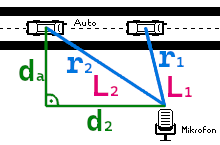
\includegraphics[width=.4\linewidth]{SchalldruckpegelSymbolbild}
    \caption{Symbolbild Schalldruckpegel und Abstand (\(d_{a}\): Abstand zur Straße)}
    \label{img:SchalldruckpegelSymbolbild}
\end{figure}

\(d_{a}\) ist hierbei der Abstand des Mikrofons zur Straße. Wenn \(d_{a}\) jedoch unbekannt ist, kann keine Geschwindigkeitsberechnung vorgenommen werden, selbst bei der Annahme, dass der Abstand des Mikrofons zur Straße vernachlässigbar ist (\(d_{a} \approx 0\)).

Dieses Problem kann an folgendem Gedankenexperiment veranschaulicht werden: Eine Schall\-druck\-pegel-Änderung um \(+6 dB\) kann interpretiert werden als ein Fahrzeug,
\begin{enumerate}
    \item welches sich von \(200 m\) zu \(100 m\) Entfernung (\(100 m\) Entfernungsunterschied) innerhalb der Zeit \(\Delta t\) angenähert hat.
    \item welches sich von \(100 m\) zu \(50 m\) Entfernung (\(50 m\) Entfernungsunterschied) innerhalb der gleichen Zeit \(\Delta t\) angenähert hat.
\end{enumerate}
Dies hätte zur Folge, dass für das Fahrzeug aus Beispiel \((1)\) die doppelte Geschwindigkeit \(v\) wie für Fahrzeug \((2)\) berechnet würde, da es keinen Referenzwert gibt.

Bei bekanntem Abstand zur Straße kann die Aufnahme auf Hochpunkte im Schalldruckpegel untersucht werden. Der Hochpunkt stellt dann den Moment der geringsten Distanz zwischen Mikrofon und Fahrzeug dar. Damit wird die Unbekannte \(r_{1}\) in \autoref{equation:RadiusAusSchallpegel} durch \(d_{a}\) ersetzt und die Unbekannte ist eliminiert. Durch eine Normalisierung der Audiorohdaten auf \(-0 dB\) kann dann für \(L_{1}\) selbiger Gleichung \(L_{1} = 0 [dB]\) eingesetzt werden, was eine weitere Unbekannte eliminiert. Nun muss lediglich der Schalldruckpegel \(L_{2}\) aus den Audiodaten berechnet werden, um den Abstand \(r_{2}\) zu ermitteln.


\subsubsection{Versuch zur Bestimmung der Beziehung zwischen Lautstärke und Abstand}

\begin{figure}[h]
    \begin{subfigure}{.5\textwidth}
        \centering
        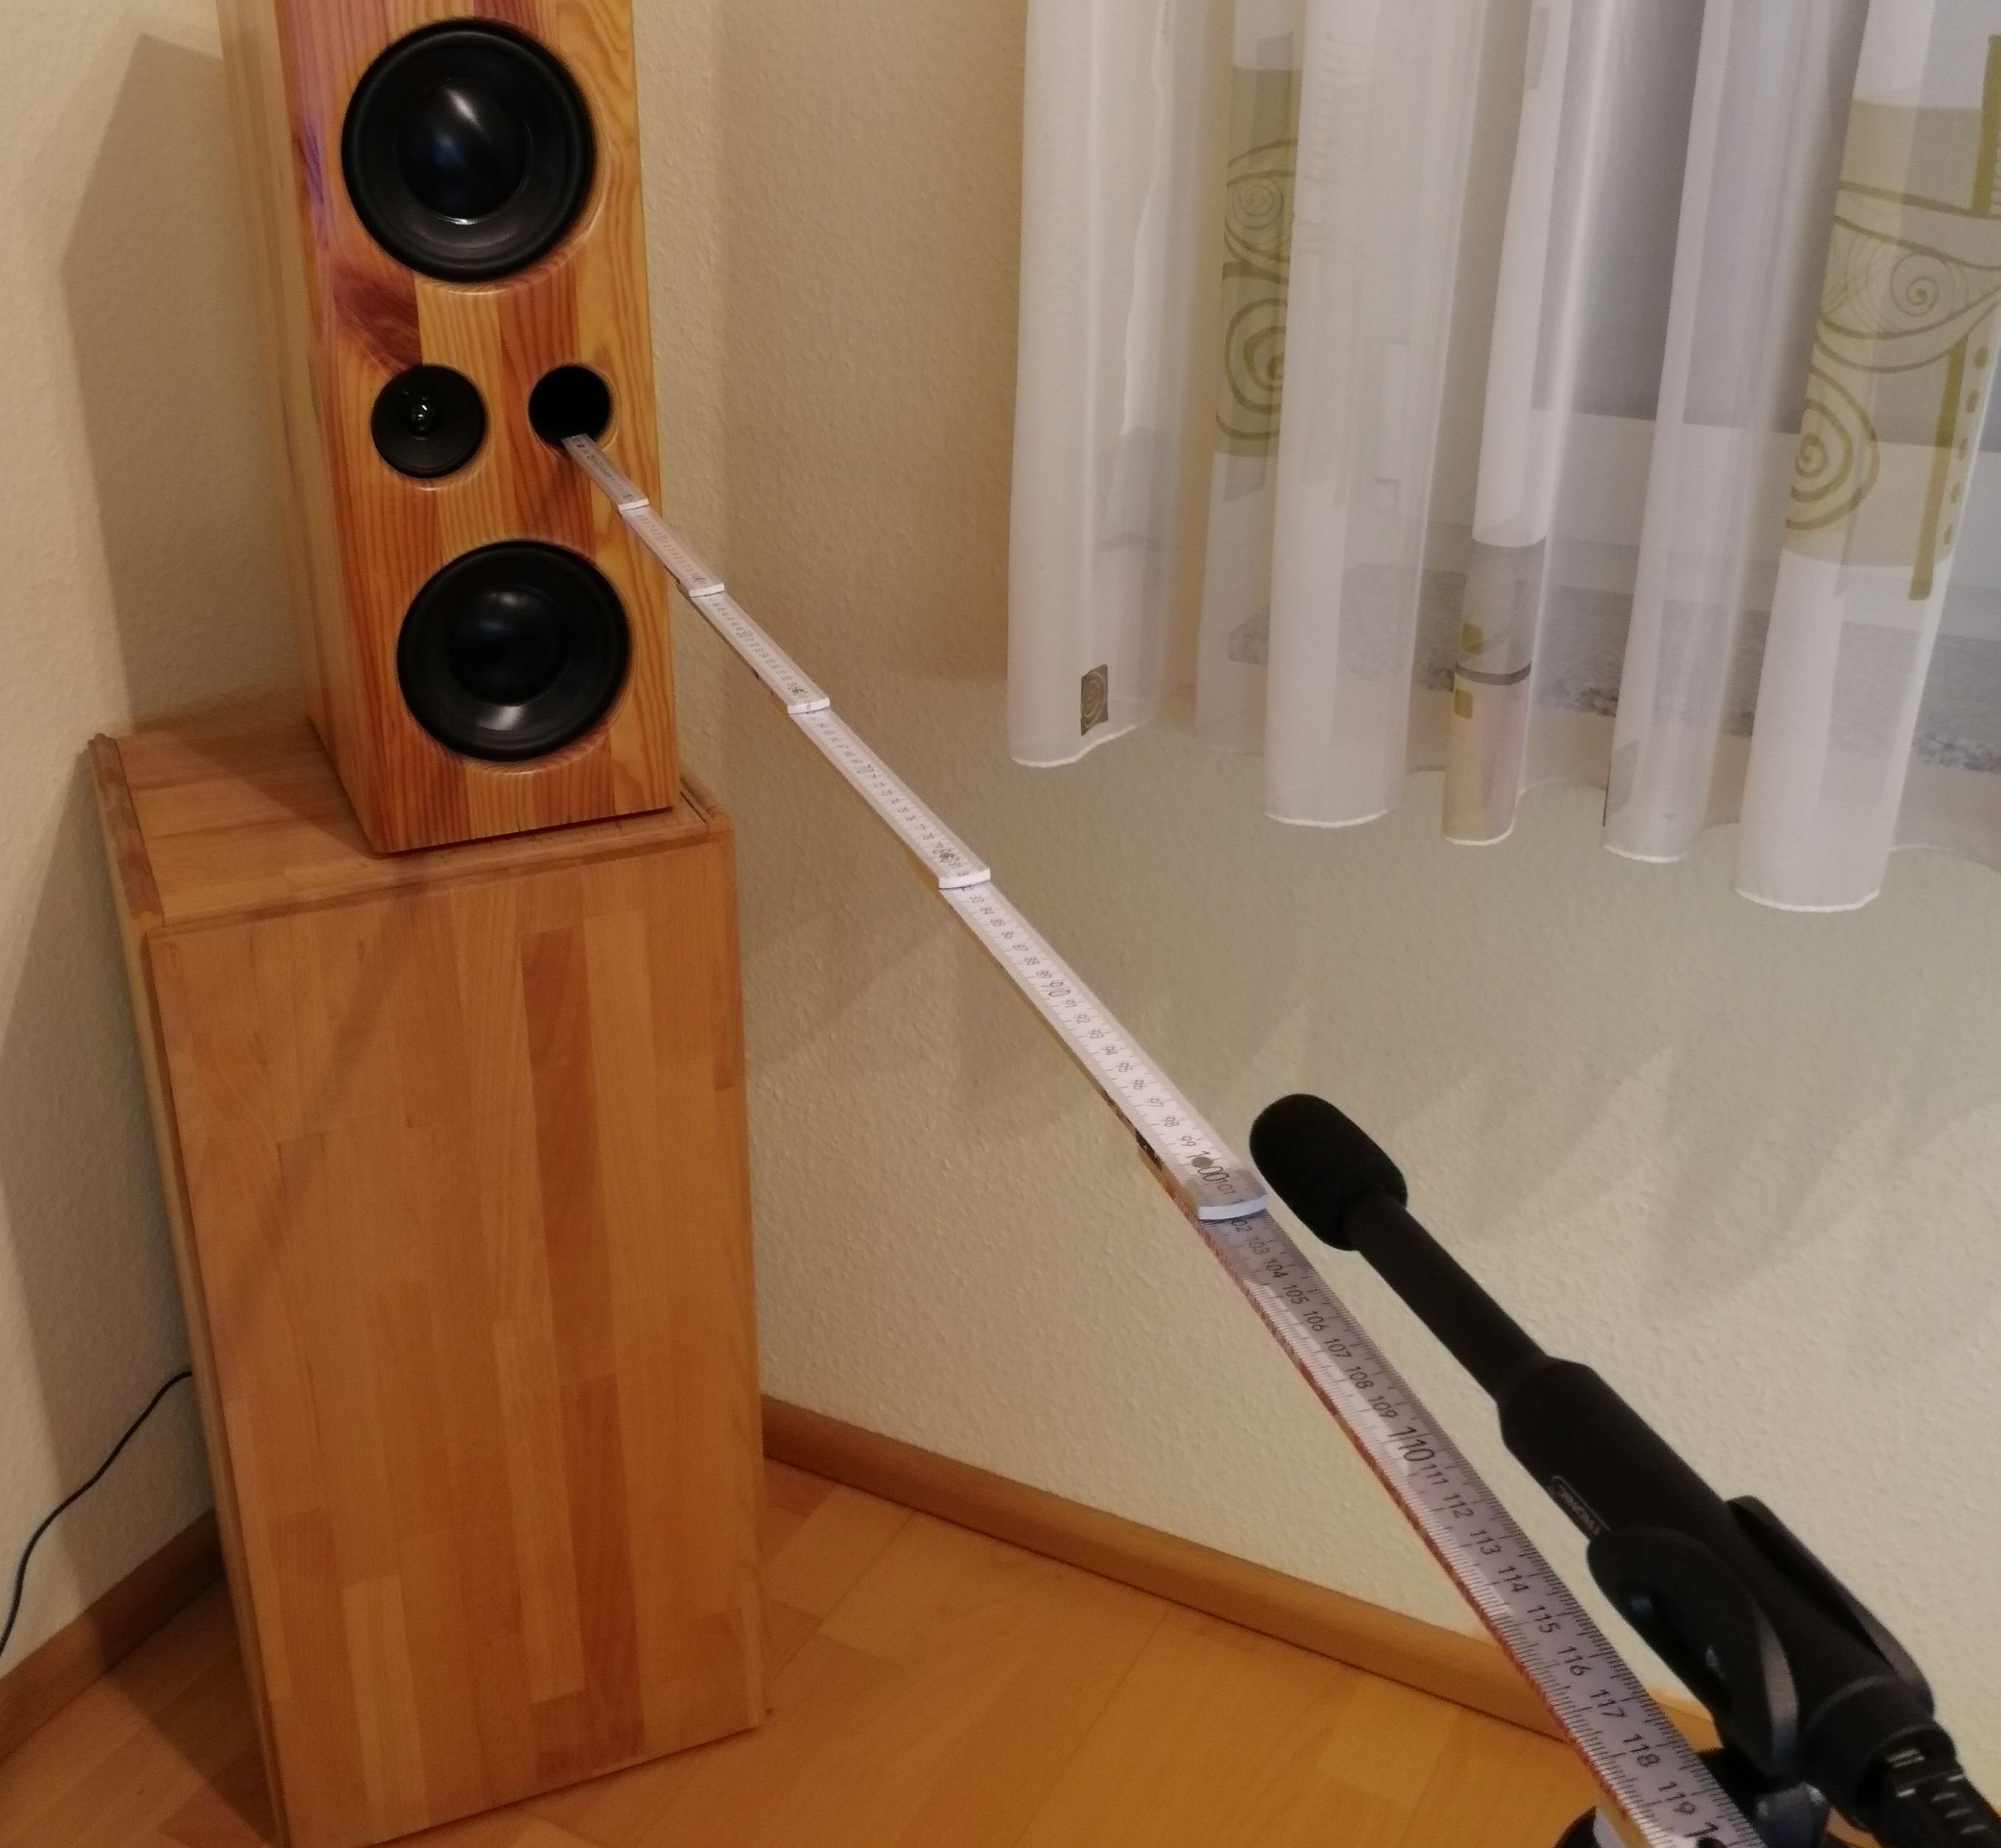
\includegraphics[width=.8\linewidth]{VersuchsaufbauAbstandInnen}
        \caption{Innenraum}
        \label{img:dist_room}
    \end{subfigure}
    \begin{subfigure}{.5\textwidth}
        \centering
        \includegraphics[width=.95\linewidth]{VersuchsaufbauAbstandsmessung_downscaled}
        \caption{Im Freien}
        \label{img:dist_free_field}
    \end{subfigure}
    \caption{Versuchsaufbau zur Lautstärkebestimmung}
    \label{img:versuche_abstand}
\end{figure}

Zuerst wurde eine Messreihe zum Verhältnis zwischen Lautstärke und Abstand im Innenraum durchgeführt. Hierfür wurde ein im Eck stehender Lautsprecher und ein Messmikrofon auf einem Stativ gegenübergestellt (siehe \autoref{img:dist_room}). Bei verschiedenen Abständen wurde zunächst ein \(1 kHz\)-Ton über den Lautsprecher abgespielt und vom Mikrofon aufgenommen. Bei der Auswertung der Messergebnisse stellte sich heraus, dass der Innenraum bei bestimmten Abständen die Töne „verschluckt“, da durch Reflexionen der Schallwelle an den Innenwänden des Raumes an diesen Punkten eine destruktive Interferenz entsteht. Da das Interferenzmuster von der Frequenz der Schallwelle abhängt, wurde anschließend der gleiche Versuch mit einem weißen Rauschen als ausgesendetes Geräusch verwendet, um durch das breite Frequenzspektrum die Tiefpunkte der Lautstärke zu vermeiden. Zur Berechnung des effektiven Schalldruckpegels wurde das Programm „Audacity“ \cite{Audacity} und dessen „Measure RMS“-Funktion verwendet.

Bei der Auswertung der Aufnahmen stellte sich heraus, dass für Abstandsverdoppelung der Schalldruckpegel um etwa \(4 dB\) absank, was nur zwei Drittel der erwarteten Absenkung entspricht. Diese Abweichung lässt sich auf den Versuchsaufbau zurückführen: Der Lautsprecher stellt in seiner aktuellen Aufstellung eine gerichtete Schallquelle dar, der verwendete Innenraum ist nicht reflexionsarm. Beides sind Ausschlusskriterien für die Anwendbarkeit des reziproken Abstandsgesetzes, da der Pegelabfall dadurch geringer ausfällt.

Um beide Probleme zu beheben, wurde ein zweiter Versuch durchgeführt. Dieser fand im Freien statt, um Reflexionen an Wänden zu vermeiden. Zudem wurde der verwendete Lautsprecher mit seiner Membran (Chassis) nach oben ausgerichtet, das Mikrofon wurde für die Entfernungsmessung jedoch weiterhin in der Horizontalen bewegt. Somit kann die Schallquelle näherungsweise als Quelle mit kugel- bzw. halbkugelförmiger Charakteristik betrachtet werden, ähnlich wie es ein vorbeifahrendes Fahrzeug darstellt. \cite{SengpielDirektUndRaumfeld} Es wurden drei Messreihen aufgestellt, die ersten beiden davon mit gleicher Ausgabeamplitude des Lautsprechers, die dritte mit geringerer Amplitude.

\begin{figure}[h]
    \begin{subfigure}{.5\textwidth}
        \centering
        \import{rsc/plots/d-L-plot/}{abstand-pegel-plot.tex}
        \caption{Rohdaten}
        \label{fig:pegelplot_roh}
    \end{subfigure}
    \hfil
    \begin{subfigure}{.5\textwidth}
        \centering
        \import{rsc/plots/d-L-plot/}{d-L-avg-plot.tex}
        \caption{Mittelwert und Vergleichsfunktion}
        \label{fig:pegelplot_avg}
    \end{subfigure}
    \caption{Auswertung der Versuchswerte}
\end{figure}

In \autoref{fig:pegelplot_roh} sind die aufgenommenen, auf \(-0 dB\) normierten Rohdaten aller Messreihen. Diese werden in \autoref{fig:pegelplot_avg} mit der Logarithmus-Funktion für den Bezug von Schalldruckpegel und Distanz verglichen. Es fällt auf, dass die gemittelte empirisch gewonnene Pegelfunktion fast identisch mit der Logarithmus-Funktion ist, wodurch der Zusammenhang der Pegelabnahme um sechs Dezibel pro Abstandsverdoppelung bestätigt ist.

\subsection{Entwicklung der Software zur Auswertung der Audiodaten}
\label{section:EntwicklungSoftware}

Für die Auswertung wurde auf die Programmiersprache Python \cite{Python} in Kombination mit sogenannten Jupyter-Notebooks \cite{ProjectJupyter} zurückgegriffen. Python ist besonders gut für Data Science geeignet, da es viele darauf spezialisierte Pakete (Programmerweiterungen) beinhaltet und zudem effizient geschrieben werden kann. Für die Audio-Auswertung wurde hauptsächlich das Mathematik-Paket „NumPy“ \cite{NumPy} sowie die Plot-Bibliothek „Matplotlib“ \cite{Matplotlib} verwendet.

Die Auswertung der Audiodaten geschieht in drei Schritten:
\begin{enumerate}
    \item Analyse der Amplitude im zeitlichen Verlauf
    \item Annähern einer Kurve (Hyperbelfunktion) auf die Amplitudenkurve
    \item Auswertung der Amplitudenfunktion und Berechnung der Geschwindigkeit
\end{enumerate}

\subsubsection{Analyse der Amplitude im zeitlichen Verlauf}
\label{section:AnalyseAmplitude}
In diesem ersten Schritt werden die Rohdaten der aufgenommenen Audio-Datei in wenige diskrete Messpunkte heruntergebrochen, um eine weitere Analyse zu ermöglichen. Dabei musste darauf geachtet werden, dass möglichst wenig Information verloren geht.

Die Audio-Datei wird als Liste (Array) von Messpunkten eingelesen und dann weiterverarbeitet. Der genaue Ablauf ist in \autoref{fig:flow_amp_analyser} dargestellt.

\begin{figure}[h]
    \centering
    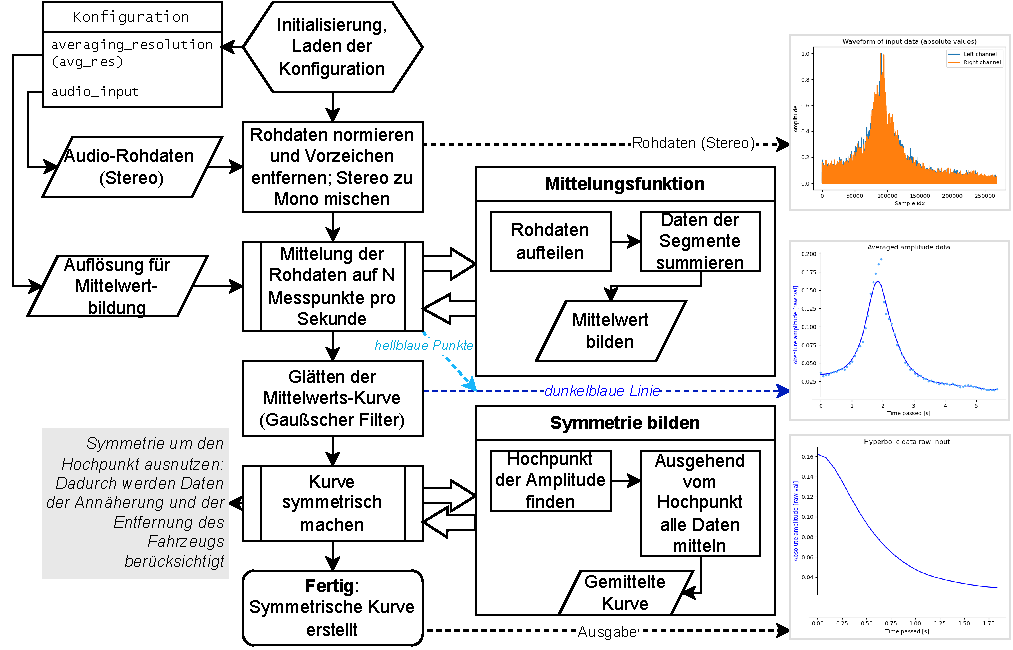
\includegraphics[width=\textwidth]{AmplitudeAnalyser.pdf}
    \caption{Flussdiagramm zur Verarbeitung der Rohdaten, \(N\) empirisch ermittelt}
    \label{fig:flow_amp_analyser}
\end{figure}

\begin{figure}[h!]
    \begin{subfigure}{.45\textwidth}
        \centering
        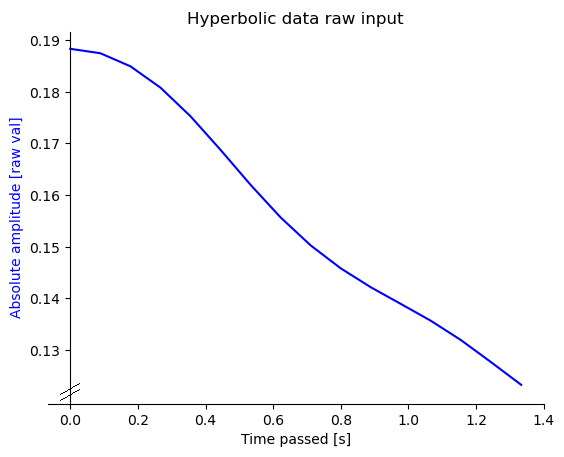
\includegraphics[width=.8\linewidth]{avg_symm_faulty}
        \caption{Gemittelte Rohdaten}
        \label{img:avg_symm_faulty}
    \end{subfigure}
    \begin{subfigure}{.45\linewidth}
        \centering
        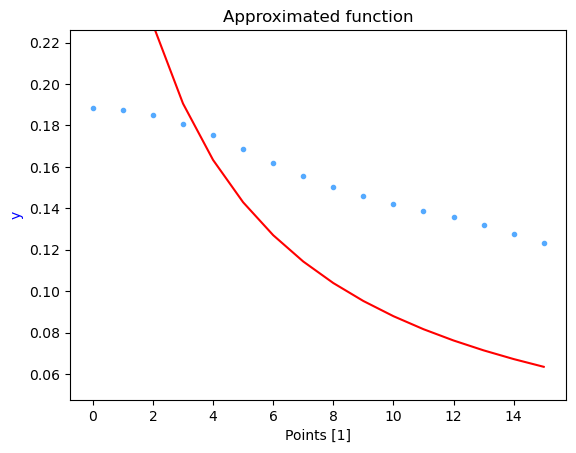
\includegraphics[width=.8\linewidth]{approx_function_faulty}
        \caption{Fehlerhafte angenäherte Funktion}
        \label{img:approx_function_faulty}
    \end{subfigure}
    \caption{Unbrauchbare Daten aufgrund von Mittelung}
    \label{img:faulty_averaging}
\end{figure}

Es stellte sich jedoch heraus, dass in einigen Aufnahmen die Mittelung von Annäherung und Entfernung sowie die Mittelung beider Stereokanäle ungeeignet ist (Beispiel siehe \autoref{img:faulty_averaging}). Der Mittelwert-Ansatz wurde deshalb verworfen, stattdessen wurden in der nächsten Version insgesamt vier Einzelkurven berechnet, pro Kanal eine für die Annäherung und eine für die Entfernung des Kfz. Der Einfachheit halber wird bei den folgenden Abbildungen nicht berücksichtigt, dass immer insgesamt vier Datenreihen verarbeitet werden.

Die Punkte der gemittelten Rohdaten werden im nächsten Schritt an die Kurvenannäherung weitergegeben.

\FloatBarrier
\subsubsection{Annäherung der Hyperbelfunktion}
Für die Vereinfachung der Geschwindigkeitsberechnung wird im nächsten Schritt auf die gemittelten Rohdaten eine Hyperbelfunktion angenähert, da sich der Schalldruck umgekehrt proportional zum Abstand von Messgerät und Schallquelle verhält, wie in \autoref{section:AnalyseAudiodatenPegel} bereits beschrieben. Ausschlaggebendes Merkmal einer Hyperbel \(f(x) = a * \frac{1}{x}\) ist deren Streckfaktor \(a\). Im konkreten Anwendungsfall existiert keine Verschiebung der Funktion entlang der x-Achse, da der Hochpunkt der Rohdaten an der Stelle \(x = 0\) liegt. Ebenso wird die Verschiebung entlang der y-Achse nicht berücksichtigt, da der hyperbelförmige Teil der Aufnahme einer nicht verschobenen Funktion entspricht.

Der Annäherungsalgorithmus funktioniert prinzipiell mit jeder beliebigen mathematischen Funktion und besteht aus zwei wesentlichen Teilen:
\begin{enumerate}
    \item Eine Gütefunktion bestimmt die Abweichung der approximierten Funktion zu den Messwerten.
    \item Über einen rekursiven Ansatz wird das Extremwertproblem gelöst, die Güte zu maximieren beziehungsweise die Abweichung zu minimieren.
\end{enumerate}

Die Gütefunktion gewichtet dabei Werte mit größerem $x$-Wert stärker, da die Rohdaten aufgrund der \emph{nicht} unendlich groß werdenden Amplituden nahe \(0\) keiner Hyperbel mehr entsprechen. Das ist gleichzeitig eine Grenze des Annäherungs-Ansatzes.

\autoref{fig:flow_curve_fitter} beschreibt vereinfacht den rekursiven Ablauf der Annäherung des Hyperbel-Streckfaktors.

\begin{figure}[h]
    \centering
    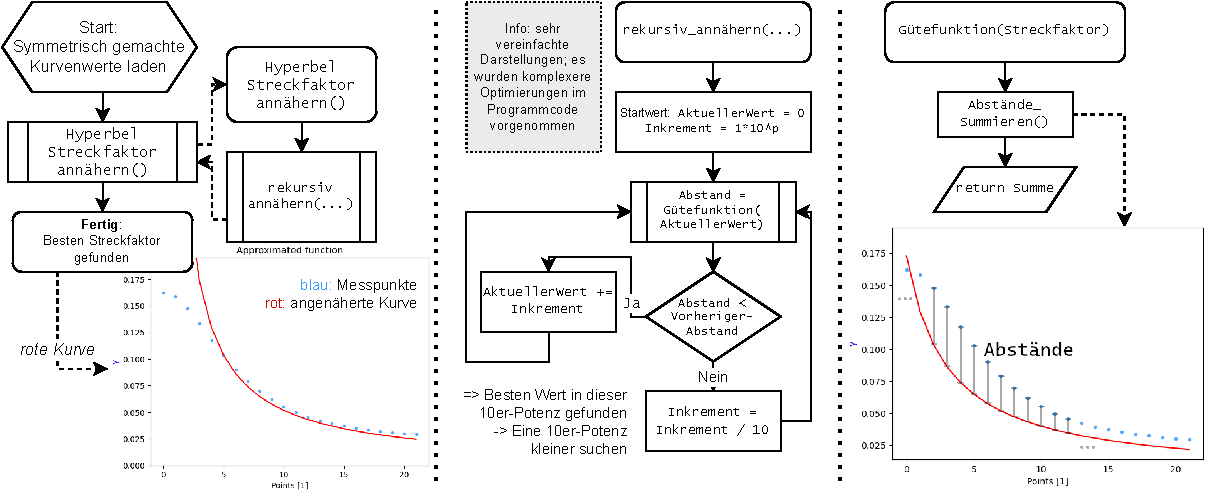
\includegraphics[width=\textwidth]{CurveFitter.pdf}
    \caption{Flussdiagramm zur Annäherung der Hyperbel}
    \label{fig:flow_curve_fitter}
\end{figure}

In \autoref{fig:ex_hyperbel_approx} wurde anhand eines trivialen Beispiels der Ablauf der Annäherung dargestellt. Das Beispiel ist trivial, da „Abstand“ hier den Abstand der aktuellen Annäherung („Versuch“) auf dem Zahlenstrahl darstellt. Bei der Annäherung der Hyperbel wird der „Abstand“ jedoch von einer Gütefunktion berechnet, wie in \autoref{fig:flow_curve_fitter} (rechts) dargestellt.

\begin{figure}[h]
    \centering
    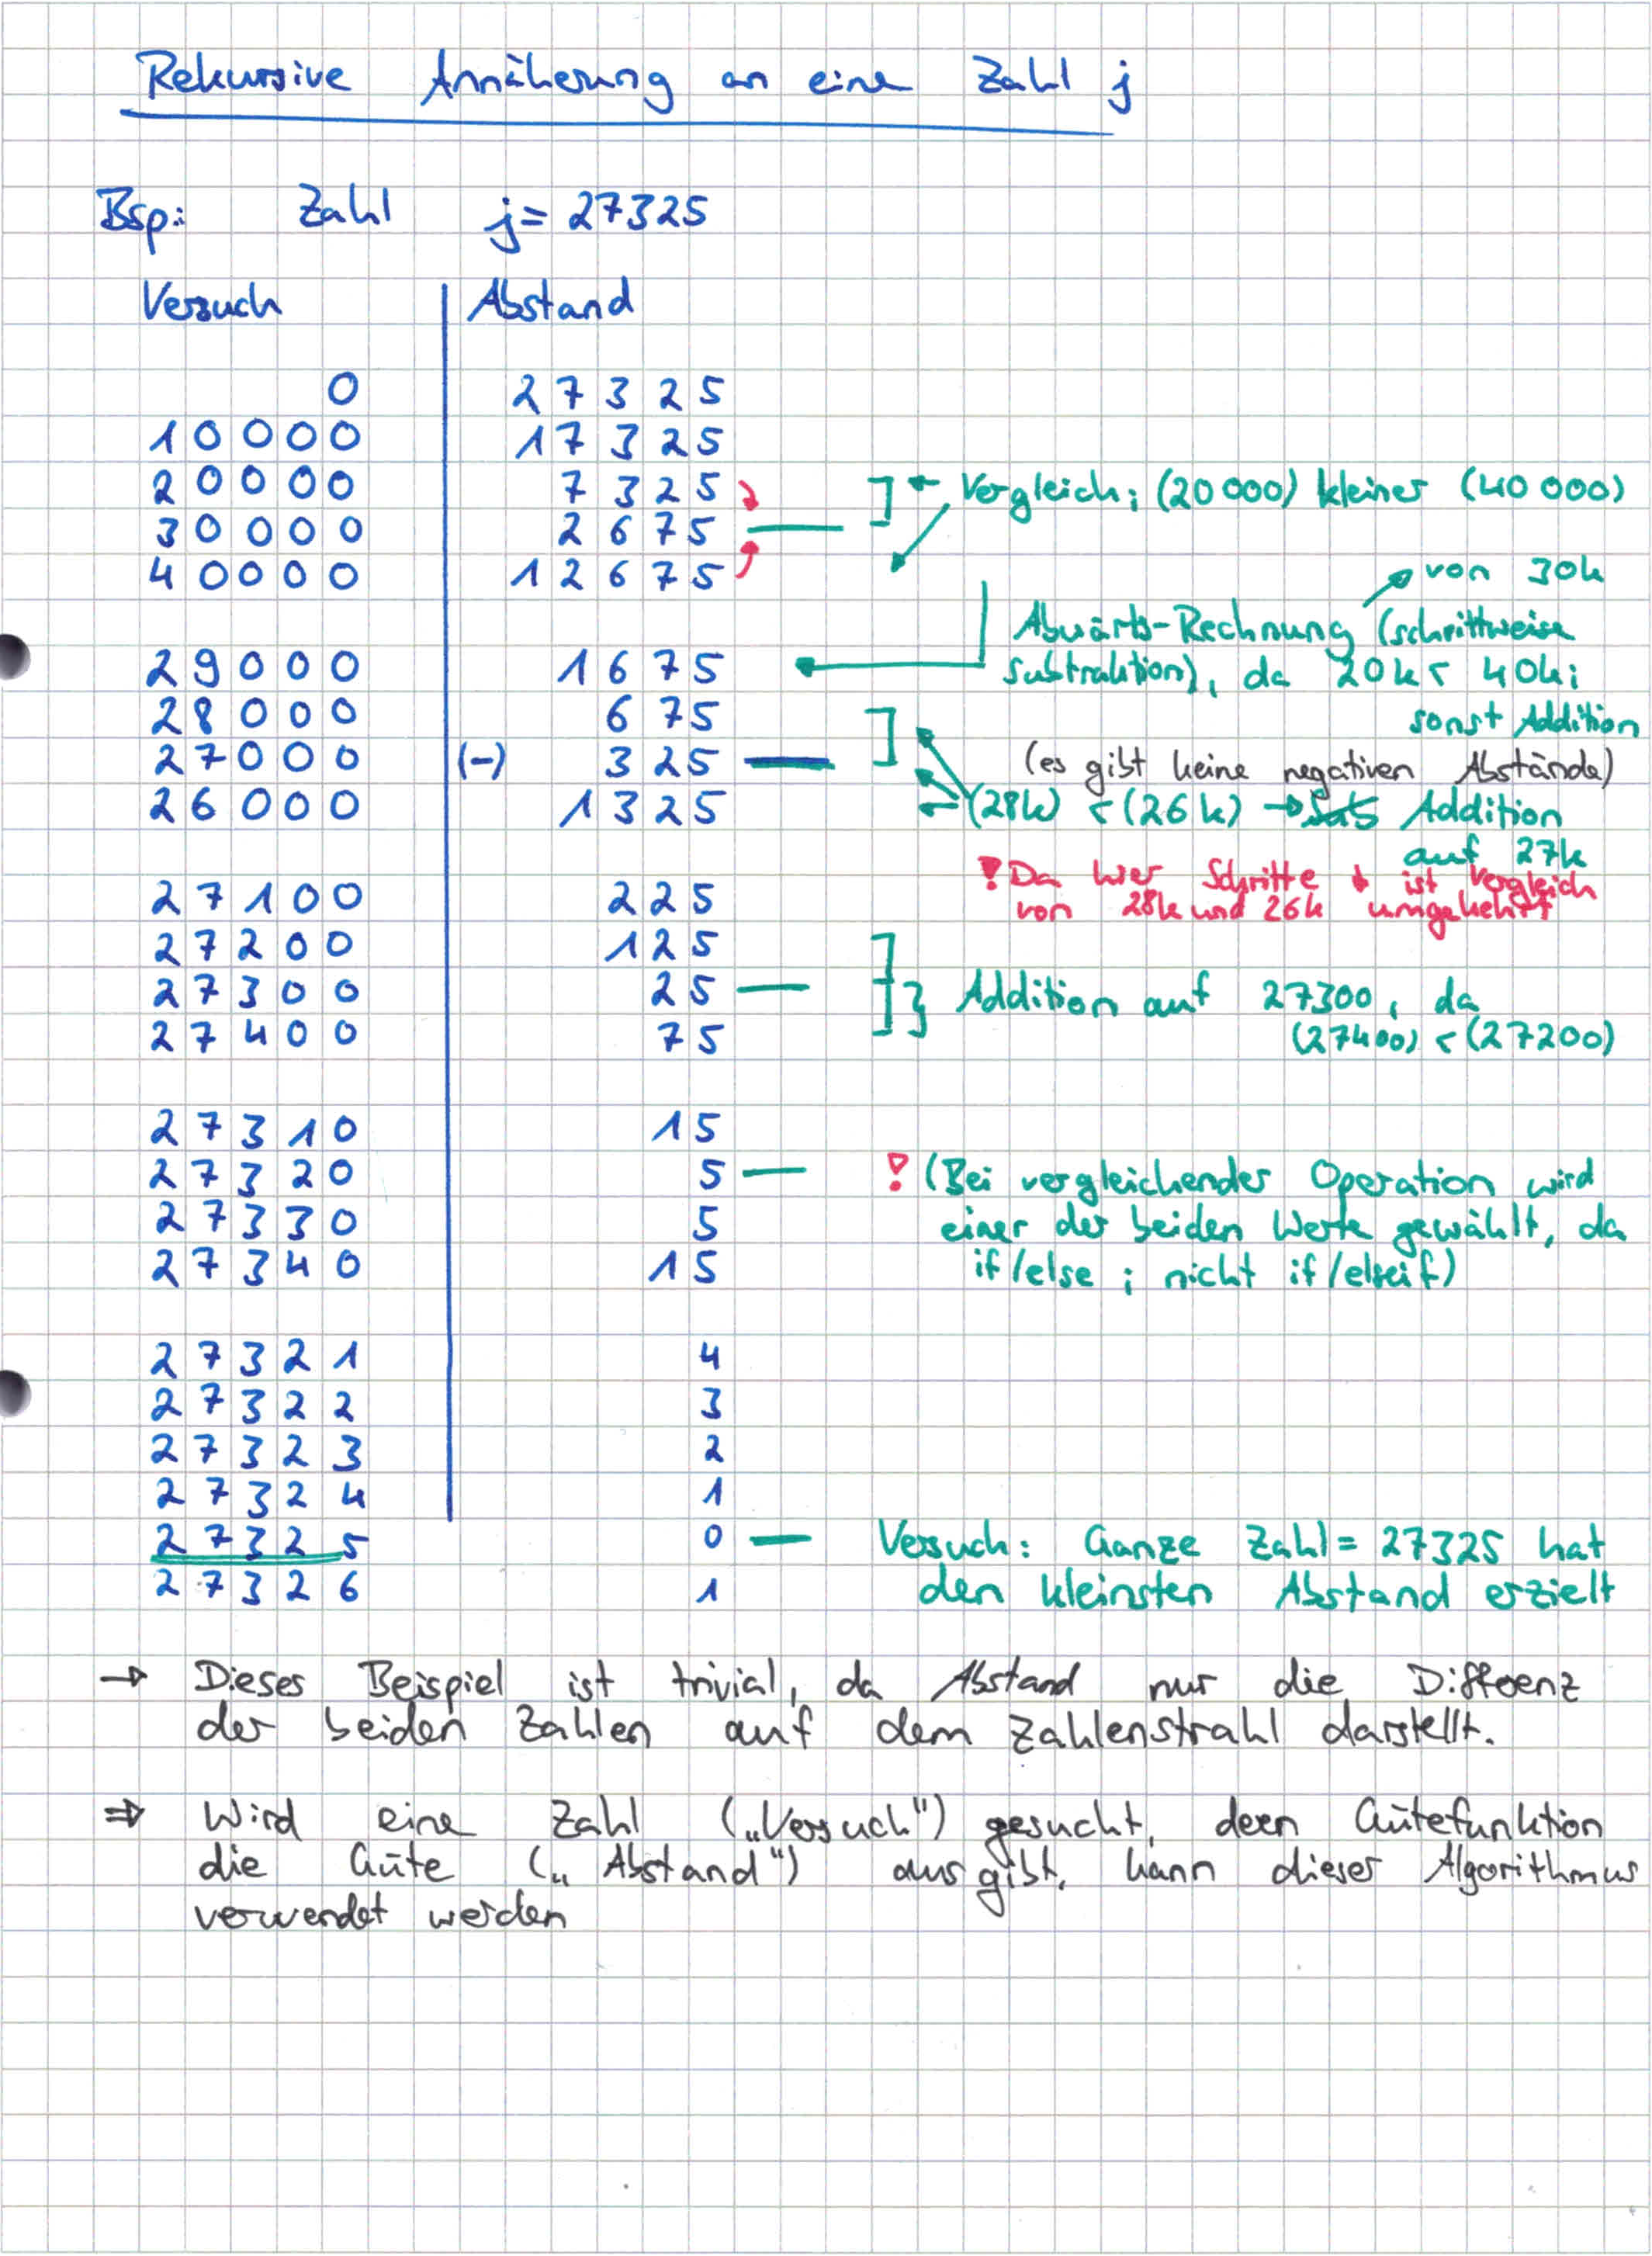
\includegraphics[width=\textwidth]{HyperbelApproxBsp}
    \caption{Triviales Beispiel zur Annäherung der Hyperbel}
    \label{fig:ex_hyperbel_approx}
\end{figure}

\FloatBarrier
\subsubsection{Geschwindigkeitsberechnung}
Im dritten Schritt wird zunächst die Amplitudenfunktion in eine Funktion des effektiven Schalldruckpegels (RMS) über Zeit umgerechnet. Diese Umrechnung geschieht in zwei Schritten: Zuerst wird der Effektivwert (Root Mean Square, RMS) der Amplitude berechnet \cite{SiemensRMS}, um nicht in Grenzfälle, wie \(a = 0 \longrightarrow L(0) = -\infty\), zu geraten. Anschließend wird die Amplitude in einen Pegel umgerechnet, da bei Pegeln die „\(6 dB\)-Abstandsregel“ angewendet werden kann.
\begin{equation}
    \begin{split}
        L_{amplitude}(a) = 20 * \log(a) \\
        L_{RMS}(a) = L_{amplitude}\left(\sqrt{\frac{a^2}{2}}\right)
    \end{split}
    \label{equation:LRMS}
\end{equation}

Für eine Geschwindigkeitsberechnung bei näherungsweise gleichförmiger Bewegung des vorbeifahrenden Fahrzeugs kann die Formel \(v = \frac{\Delta s}{\Delta t}\) verwendet werden. Für die Berechnung des Wegunterschieds wird zweimal auf \autoref{equation:RadiusAusSchallpegel} zurückgegriffen, um die Abstände von Mikrofon und Fahrzeug an zwei beliebigen Punkten der angenäherten Hyperbel-Kurve zu berechnen. Die Wahl der Punkte spielt hierbei keine Rolle, da die Pegelfunktion einer reinen Logarithmusfunktion entspricht, weil diese aus der angenäherten Hyperbel und nicht aus Rohdaten berechnet wurde. Der Einfachheit halber und um Rundungsfehler zu minimieren, wurden die Punkte bei \(x_{2} = \frac{1}{3} * len, \quad x_{3} = \frac{2}{3} * len\) für die Berechnung gewählt sowie der Referenzwert \(x_{1} = d_{a}\) (\(d_{a}\): Abstand vom Mikrofon zur Straße) mit \(L_{1} = 0 dB\). \(len\) ist hierbei die Länge der Liste der Messpunkte.

Mithilfe von \autoref{equation:RadiusAusSchallpegel}:
\begin{equation*}
    \begin{split}
        r_{2} = r_{1} * 10^{\left(\frac{\abs{L_{1} - L_{2}}}{20}\right)} \\
        d_{2} = \sqrt{r_{2}^2 - d_{a}^2}
    \end{split}
\end{equation*}
kann für \(r_{1} = d_{a}\) und für \(L_{1} = 0 dB\) eingesetzt werden. \(L_{2}\) wird daraufhin aus der Funktion des effektiven Schalldruckpegels (\autoref{equation:LRMS}) an den Stellen \(x_{2}\) und \(x_{3}\) berechnet und eingesetzt. Die beiden berechneten Abstände \(d_{2}\) und \(d_{3}\) werden verwendet, um die Geschwindigkeit zu berechnen:
\[
    v_{2,3} = \frac{d_{3} - d_{2}}{\Delta t_{2,3}}
\]

Da \(d\) üblicherweise in Metern und \(t\) in Sekunden angegeben wird, muss für eine Geschwindigkeit in Kilometern pro Stunde \(v_{2,3}\) noch mit \(3,6\) multipliziert werden. Somit wurde die Geschwindigkeit \(v\) eines vorbeifahrenden Fahrzeugs anhand der Lautstärkeänderung berechnet.